\begin{appendices}
\section {TWIN MUSIC Geometric Acceptance Correction via Efficiency Measurement}
Instead of correcting the limited geometric acceptance of TWIN MUSIC via graphical fitting (see section \ref{sec:geo_corr}) it is also feasible correcting via TWIN MUSIC efficiency measurement. The correction factor is given by:
\begin{equation}\label{eq:twin_eff}
\epsilon_{geo\text{\_}corr} = \frac{N_{MWPC1,MWPC2}}{N_{MWPC1,MWPC2,TWIN}}
\end{equation}
where $N_{MWPC1,MWPC2}$ corresponds to the number of events with a hit in MWPC1 and MWPC2 whereas $N_{MWPC1,MWPC2,TWIN}$ imposes the further condition having a hit in TWIN MUSIC too.\newline
The corresponding correction factor $\epsilon_{geo\text{\_}corr}$ is consequentely applied on all target and empty runs. The resulting corrected charge changing cross section is shown in figure \ref{fig:twim_corr_cc_cs}. 
\begin{figure}[h!]
    \centering
    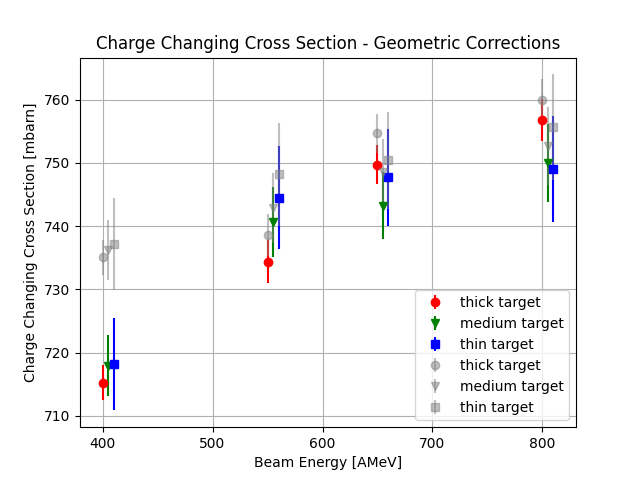
\includegraphics[width=\textwidth,height=8cm,keepaspectratio=true]{Figures/charge_changing_cross_sec_twim_eff_corr.png}
    \caption{
        Charge changing cross section correction due to limited geometric acceptance of TWIN MUSIC via efficieny correction with MWPC1 and MWPC2. In gray: charge changing cross section measurements before applying corrections, as in figure \ref{fig:cccs_gaus_diff_sections}}
    \label{fig:twim_corr_cc_cs}
\end{figure}
The same correction factor can be applied to the total interaction cross section as in figure \ref{fig:twim_corr_tot_cs}. 
\begin{figure}[h!]
    \centering
    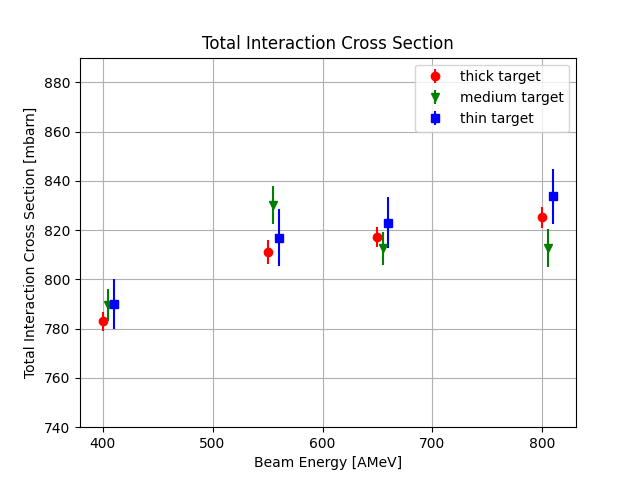
\includegraphics[width=\textwidth,height=8cm,keepaspectratio=true]{Figures/tot_interaction_cs_twim_eff_corr.png}
    \caption{
        Total interaction cross section of $^{12}$C + $^{12}$C using the TWIN MUSIC efficiency correction factor, see equation \ref{eq:twin_eff}, to compensate for the limited geometric acceptance in TWIN MUSIC.}
    \label{fig:twim_corr_tot_cs}
\end{figure}
\newpage


\section{appendix-test}
foo test appencdix of qfs
\section {second stuff I want to add}\label{appendix_first}
hello here to add, end.
\end{appendices}
